\chapter{Cyber War e attacchi ad infrastrutture critiche}
La cyber war è una guerra condotta tramite reti e computer. Di solito coinvolge due paesi, dove l'attaccante impiega un gruppo di hacker per sabotare strutture critiche dell'altro paese tramite cyber weapons (solitamente malware molto specializzati). 

Un gruppo di hacker nord koreano che effettua un attacco DDoS a uno dei maggiori provider telefonici americani NON è un attacco di cyber war. Un attacco di cyber war dovrebbe avere un impatto sulla vita sociale/economica/politica della nazione colpita. 
Un gruppo di hacker cinese che attacca una stazione elettrica americana può essere considerato un attacco di cyber war, in quanto l'obiettivo è una struttura critica e l'assenza della corrente elettrica ha un grande impatto sulla vita dei cittadini.

\paragraph{Infrastrutture critiche} Infrastrutture, sistemi, siti, informazioni, persone, reti o processi necessari al funzionamento e vita di una nazione. Comprendono anche quelle organizzazioni, persone e siti che non sono critici al mantenimento dei servizi essenziali, ma la cui protezione è necessaria a causa del grande pericolo che possono provocare al pubblico (es: nucleare civile, siti chimici).

\paragraph{Elenco strutture critiche} Trasporti pubblici, rete elettrica, comunicazione difesa, servizi di emergenza, finanza, salute, centrali nucleari, ...

\paragraph{Principali pericoli} Poiché queste infrastrutture forniscono servizi vitali per la vita di tutti i giorni, sono interessato a garantirne la disponibilità, l'integrità e la safety (es: attacco che modifica la velocità della turbine per farla esplodere -> può ferire gli operatori vicini). In figura \ref{fig:my_label4} sono riportati alcuni dei principali attacchi conosciuti.

\begin{figure}
    \centering
    
\includegraphics[width=1\textwidth]{images/6.png}
    \caption{Principali attacchi alle infrastrutture critiche}
    \label{fig:my_label4}
\end{figure}

\section{Sistemi di controllo industriale}

La maggior parte delle strutture critiche sono controllate e monitorate da sistemi di controllo industriale (ICS), che garantiscono la sefaty e la disponibilità. 

\paragraph{Componenti degli ICS} Ho uno o più processi da monitorare (produrre una macchina, sollevare la sbarra del parcheggio, produrre energia elettrica), implementati su macchine a cui sono associati sensori, che ne catturano i dati sul funzionamento. I dati cono verificati da un controllore. Il sistema di controllo industriale implementa due tipi di controllori: 
\begin{itemize}
    \item Uno più vicino alle macchine, che implementa il processo di controllo industriale. Prende il nome di Program Logic Controller (PLC) - quello che posso vedere con \href{https://shodan.io}{https://shodan.io};
    \item Uno più distribuito, chiamato SCADA, che controlla tutti i dispositivi coinvolte nel processo industriale.
\end{itemize}

Il controllore comunica con la Human Machine Interface (HMI), che è l'interfaccia usata dall'operatore. L'operatore invia dei comando al controllore, che li inoltra agli attuatori.

\paragraph{Sistemi SCADA} Tra i sistemi più diffusi, è un sistema distribuito consiste di un server che comunica con più stazioni (es: quelle per la distribuzione dell'energia elettrica locali di ogni città) e ne raccoglie i dati. I dati raccolti vengono salvati in un Data Historian ed utilizzabili dagli operatori in caso di necessità. Gli operatori possono anche, tramite le Engineering Workstation, inviare comandi alle diverse stazioni. Un esempio di dispositivo che posso trovare nelle stazioni locali sono gli interruttori per trasmettere l'energia elettrica 

Questi sistemi presentano diverse vulnerabilità. 

La più importante è legata al fatto che  inizialmente questi sistemi erano chiusi, quindi non connessi alla rete. Ora sempre di più utilizzano connessioni internet normali per funzionare. Questo li espone logicamente ad una serie di attacchi.

Molto spesso, inoltre, per garantire la disponibilità dei servizi, il ciclo di vita del macchianario viene estessa molto (circa 10-20 anni). Quindi molti dei sistemi in uso utilizzano sw obsoleti non più supportati dal venditore.

Un'altra problematica è legata all'accesso a questi dispositivi. Molti dei sistemi di autenticazione utilizzano l'autenticazione con password, che viene spesso lasciata a quella di default.

Spesso non vengono mantenuti log delle attività svolte dai vari sipositivi, rendendo quindi difficile ricostruire gli attacchi subiti.

\section{Cyber kill chain per attacchi ICS}

Per gli attacchi agli ICS è stata sviluppata una cyber kill chain specifica. Secondo la ricerca svolta, questa si compone di due fasi:
\begin{itemize}
    \item La prima ha l'obiettivo di ottenere accesso alla rete dell'ICS, e segue le stesse fasi viste nella cyber kill chain classica.
    \item La seconda fase è quella in cui avviene l'attacco vero e proprio. che si divide in: sviluppo, test, consegna, installazione ed esecuzione dell'attacco all'ICS.
\end{itemize}

Supponiamo che il mio obiettivo sia modificare il sw che gira sul PLC che controlla gli interruttori che attivano/bloccano il trasferimento della corrente elettrica. Per fare ciò sviluppo un malware specifico, che posso testare sul medesimo PLC presente nella stazione che ho acquistato a priori sul mercato (il mio attacco è molto specifico, quindi devo effettuare dei test prima di metterlo in pratica). La delivery del malware la posso fare tramite campagne di phishing oppure sfruttando una chiavetta USB portata all'interno da un insider. 
	
\subsection{Esempi di attacchi reali}

\paragraph{Stuxnet} Prima cyber weapon. Può essere considerato ad oggi il malware più sofisticato mai realizzato. Sviluppato dai servizi di sicurezza americani e dell'intelligence israeliana per sabotare lo sviluppo nucleare iraniano. la cyber kill chain di Stuxnet è riportata in figura \ref{fig:my_label5}.

\begin{figure}
    \centering
    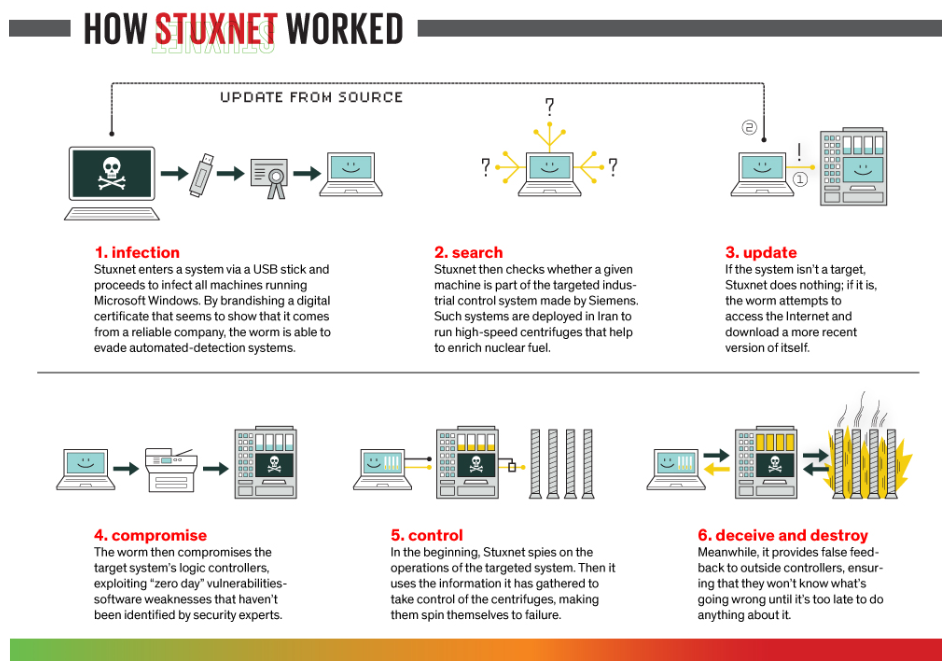
\includegraphics[width=1\textwidth]{images/7.png}
    \caption{Cyber kill chain di Stuxnet}
    \label{fig:my_label5}
\end{figure}

\noindent Stuxnet utilizza due tecniche di propagazione:
\begin{enumerate}
    \item Propagazione tramite network:
	\begin{itemize}
	    \item Infettando le macchie WinCC sfruttando hardcoded passwed (psw salvate in chiaro);
    	\item Propagandosi sfruttando la vulnerabilità zero-day MS10-061 Print;
    	\item Propagandosi sfruttando la vulnerabilità  MS08-067 del Windows Server Service;
	\end{itemize}
    \item Propagazione tramite dispositivi rimovibili, tramite:
    \begin{itemize}
        \item Vulnerabilità LNK (CVE-2010-2568);
    	\item Autoorun.inf.
    \end{itemize}
\end{enumerate}

\noindent Quando veniva infettata una chiavetta USB, venivano creati nella chiavetta tre file: un collevamento a Shortcul.lnk e due file temporanei.Quando la chiavetta veniva inserta, veniva eseguito lo shortcut, che andava a caricare il primo file tmp, che a sua volta caricava il secondo, che conteneva effettivamente il malware. 
	
Nella prima parte del file Autorun.inf c'era la copia di stuxnet. Questo è visibile dal fatto che ogni eseguibile Windows inizia con i caratteri $MZ$. 
Quando la chiavetta veniva pluggata, l'autorun rimandava all'esecuzione del programma che conteneva.
	
La parte di Commando e Control permetteva di staricare versioni aggiornate del malware, ma sembra che questa feature non sia mai stata usata.
	
Stuxnet andava a infettare pc che eseguivano il programma Step7, che consentiva di leggere e scrivere i programmi eseguiti dal PLC, e sostituiva una  libreria legittima che permetteva di modificare il codice eseguito dal PLC, e quindi lanciare comandi, con una versione malevola.
La libreria permetteva di modificare la velocità dei rotori delle turbine (per farle surriscaldare) o modificare la pressione del gas inserito (causando un aumento critico).

\paragraph{Attacchi del gruppo Sandworm} Gruppo affiliato al governo russo. I membri sono autori di diversi attacchi ad infrastrutture critiche di diversi paesi a partire dal 2015, come:
\begin{itemize}
    \item Attacco alla rete elettrica ucraina;
    \item Campagna di Spearphishing contro i membri del partito del presidente Macron (2017);
    \item Infezioni col ransomware NotPetya (2017);
    \item Attacchi contro le olimpiadi invernali (2017);
    \item Rallentamento delle investigazioni sulla morte della spia Novick (2018);
    \item Campagne contro infrastrutture critiche e siti governativi della Georgia.
\end{itemize}

\noindent Il primo attacco è stato effettuato il 23 dicembre 2015 in una stazione elettrica in Ucraina, che ha causato il blackout in una regione dei dintorni della capitale Kiev per qualche ora. Questo è stato il primo attacco ad una struttura critica.
L'obiettivo dell'attacco erano le stazioni di distribuzione dell'energia elettrica. 

Generalmente, un sistema di distribuzione si compone di una centrale che produce l'energia e la trasferisce alle stazioni di trasmissione, che ne abbassano il voltaggio e la trasferiscono agli utenti finali. Sandworm aveva compromesso gli interruttori che consentivano al trasmissione agli utenti, impedendola.

L'attacco si è strutturato come segue:
\begin{itemize}
    \item Tramite una campagna di spearphishing, ai danni del personale amministrativo e IT, gli attaccanti installano BlackEnergy 3 sulle macchine delle vittime (tamite macro malevola);
    \item BlackEnergy 3 stabilisce una connessione C2 con gli attaccante;
    \item Viene installato KillDisk nell'ambiente per rendere le macchine Windows/workstation inutilizzabili eliminando o modificando il master boot record;
    \item Viene lanciato un attacco DoS telefonico ai call center della compagna elettrica per impedire ai client di segnalare i problemi.
\end{itemize}
 \\
 
\noindent  Il 17 dicembre 2016, Sandworm ha attaccato la trasmissione dell'energia elettrica nella capitale Kiev. L'attacco è stato simile a quello precedente: mesi prima è stata effettuata nuovamente una campagna di spearphishing per ottenere accesso alla rete. Questa volta però il malware usato era Industroyer. Si tratta di un malware di complessità simile a stuxnet, ed è il secondo malware mai creato per sabotare un sistema industriale. Il suo obiettivo era quello di rendere inutilizzabili i remote terminal unit che controllavano gli interruttori per la trasmissione dell'energia elettrica. Si componeva di moduli che implementavano i quattro possibili protocolli di comunicazione che la work station degli operatori utilizzava per inviare i comandi ai remote terminal unit delle stazioni di trasmissione. Implementava anche un attacco DDoS contro i protection relay, i meccanismi che permettevano di richiudere gli interruttori in caso si verificasse una situazione anomala. 

 Industroyer aveva struttura modulare, con una main backdoor che permetteva l'accesso alla rete dell'azienda. Questa installava inoltre un'altra backdoor, utilizzata nel caso la prima fosse eliminata e scaricava due tool, uno per rubare le credenziali delle work station e l'altro per effettuare l'attacco DDoS. Il cuore del malware è rappresentato dal launcher, che implementava ed eseguiva i quattro payload che implementavano i quattro possibili protocolli di comunicazione. 
\\

\noindent NotPetya era un ransomware che colpì inizialmente l'Ucraina, per poi diffondersi in tutto il mondo. 
In Ucraina venne diffuso come update del software di contabilità fiscale M.E.Doc (molto usato nel paese): Sandworm era stata in grado di intercettare il traffico degli aggiornamenti di questo sw e ridirigerlo in un server situato in Francia, da cui installavano il malware. Una volta installato iniziava a cifrare i dati delle macchine infette. Presentava però delle stranezze rispetto ad un normale ransomware:
\begin{itemize}
    \item Usava lo stesso indirizzo bitcoin per il riscatto in ogni infezione;
    \item Richiedeva di riceve per mail la conferma del pagamento;
    \item Se la macchina aveva più dischi, generava una chiave per ciascuno;
    \item Inviava al server una stringa casuale come ID della vittima (per identificare la chiave usata);
    \item Non prevedeva una funzionalità per riceve la chiave di decifratura.
\end{itemize}



	
	
	
	
